%% 
%% This is file ejmcls.ltx - generated with MakeDist v1.0, by M. Reed 
%% 
 
\documentclass{article}

\usepackage[utf8]{inputenc}
\usepackage{lmodern}


\usepackage{geometry}                		% See geometry.pdf to learn the layout options. There are lots.
\geometry{letterpaper}                   		% ... or a4paper or a5paper or ... 
%\geometry{landscape}                		% Activate for for rotated page geometry
%\usepackage[parfill]{parskip}    		% Activate to begin subsubsections with an empty line rather than an indent
\usepackage{graphicx}				% Use pdf, png, jpg, or eps§ with pdflatex; use eps in DVI mode
								% TeX will automatically convert eps --> pdf in pdflatex		
\usepackage{fancyhdr}
\usepackage{amssymb}
\usepackage{dsfont}
\usepackage{amsmath}
\usepackage{pgfplots}
\usepackage{tikz}
\usepackage{enumerate}
\usepackage{quoting}
\usepackage{amsthm}

\usetikzlibrary{patterns}
\usetikzlibrary{decorations.text}
\usetikzlibrary{decorations.pathmorphing}

\usepackage{caption}
\usepackage{subfig}
%\usepackage{subcaption}
\usepackage{geometry}
%\geometry{top=2cm, bottom=2cm, left=2cm, right=2cm}
\geometry{margin=2cm}

\author{Gil-Arnaud Coche}
%\date{}							% Activate to display a given date or no date


\tikzset{
  pics/carc/.style args={#1:#2:#3}{
    code={
      \draw[pic actions] (#1:#3) arc(#1:#2:#3);
    }
  }
}



\numberwithin{equation}{section}

\setlength{\parindent}{0in}

\definecolor{awesomePurple}{rgb}{0.55, 0.42, 1}

\begin{document}

\newtheorem{hyp}{Hypothese}
\newtheorem*{hyp*}{Hypothese}

\pgfdeclarepatternformonly[/tikz/radius,\thickness,\size]{rings}
{\pgfpoint{-0.5*\size}{-0.5*\size}}
{\pgfpoint{0.5*\size}{0.5*\size}}
{\pgfpoint{\size}{\size}}
{
  \pgfsetlinewidth{\thickness}
  \pgfpathcircle\pgfpointorigin{\pgfkeysvalueof{/tikz/radius}}
  \pgfusepath{stroke}
}
\newdimen\thickness
\tikzset{
  radius/.initial=4pt,
  size/.store in=\size, size=20pt,
  thickness/.code={\thickness=#1},
  thickness=0.75pt
}

\newcommand{\W}{\mathcal{W}}
\newcommand{\Lin}{\mathcal{L}}
\newcommand{\G}{\mathcal{G}}
\newcommand{\N}{\mathcal{N}}
\newcommand{\diff}{\textnormal{d}}

\title{\textbf{\color{awesomePurple}Allocation optimale avec consommation du capital.}}

\author{Gil-Arnaud Coche}
\maketitle

Dans cette note, on va chercher à comprendre les points essentiels d'une allocation de richesse entre un actif risqué et un actif sans risque, sachant que l'investisseur consomme son capital sur la période. On s'intéresse d'abord au cas simple mais instructif d'un investissement de $k = 0$ à $k = 1$. On généralise ensuite à une situation de plusieurs périodes.\\

Dans toute la note, on fera l'approximation de rendements gaussiens. Pour une mise en production c'est quelque chose qui devrait être fait avec parcimonie, mais dans le contexte explicatif qui va suivre, c'est une référence correcte pour le raisonnement.

\section{Cas de deux périodes d'investissement.}\label{sec:deux-periodes}

Mettons-nous dans la peau d'un petit porteur qui a à sa disposition un capital $\W_0$ à l'instant 0. On va essayer de comprendre comment ce petit porteur pourrait répartir ce capital jusqu'à l'instant 1 entre 
\begin{itemize}
\item un actif risqué de rendement 
$$
\mu = m + \sigma\epsilon
$$
où $\epsilon$ est une loi normale centrée et réduite;
\item un actif sans risque de rendement $r$;
\end{itemize}
sachant qu'il souhaite consommer $c$ en $k = 0$.

\subsection{Le modèle}\label{sec:deux-periodes-model}

D'après la figure \ref{fig:flux-de-richesse}, le petit porteur place en l'instant $k = 0$
\begin{itemize}
\item une valeur $\psi$ dans l'actif risqué;
\item une valeur $\psi^0$ dans l'actif sans risque.
\end{itemize}
Il consomme également $c$, de sorte que sa initiale richesse $\W_0$ peut s'exprimer comme la somme de $\psi$, $\psi^0$ et de $c$
\begin{equation}\label{eq:conservation-zéro}
\W_0 = \psi + \psi^0 + c.
\end{equation}
En l'instant $k = 1$, il reçoit 
\begin{itemize}
\item une valeur $(1 + \mu)\psi$ de son placement risqué;
\item une valeur $(1 + r)\psi^0$ de son placement sans risque.
\end{itemize}
et il se verse l'intégralité de ce qu'il a (il ne réinvestit pas). \\

\begin{figure}[h!]
\centering
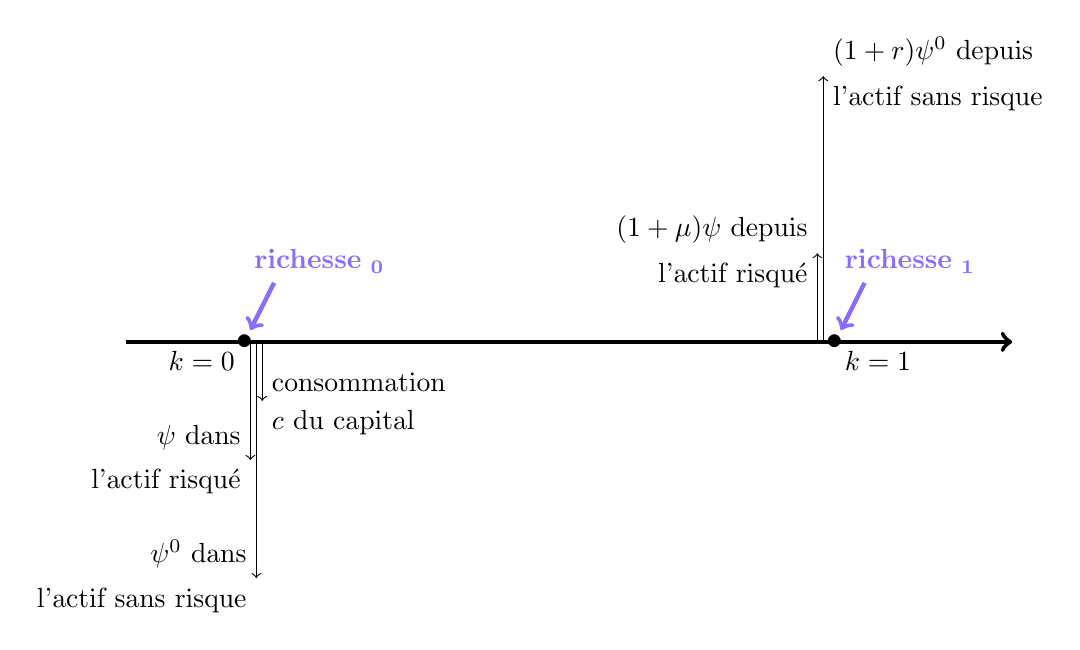
\begin{tikzpicture}[scale = .75]
\draw[->, ultra thick] (-2, 0) -- (13, 0);

\node at (0, 0) {\large $\bullet$};
\node at (0, 0) [below left] {$k = 0$};
\node at (0, 1) [above right] {\color{awesomePurple}\textbf {richesse} $\boldsymbol {\W_{0}}$};
\draw [->, ultra thick, awesomePurple] (.5, 1) -- (0.1, .2);

\node at (10, 0) {\large$\bullet$};
\node at (10, 0) [below right] {$k = 1$};
\node at (10, 1) [above right] {\color{awesomePurple}\textbf {richesse} $\boldsymbol {\W_{1}}$};
\draw [->, ultra thick, awesomePurple] (10.5, 1) -- (10.1, .2);

\draw[->] (0.1, 0) -- (0.1, - 2);
\node at (0.1, -2) [above left] {$\psi$ dans};
\node at (0.1, -2) [below left] {l'actif risqué};

\draw[->] (.2, 0) -- (.2, - 4);
\node at (.2, -4) [above left] {$\psi^0$ dans};
\node at (.2, -4) [below left] {l'actif sans risque};

\draw[->] (.3, 0) -- (.3, - 1);
\node at (.3, -1) [above right] {consommation};
\node at (.3, -1) [below right] {$c$ du capital};


\draw[->] (9.7, 0) -- (9.7, 1.5);
\node at (9.7, 1.5) [above left] {$(1 + \mu)\psi$ depuis};
\node at (9.7, 1.5) [below left] {l'actif risqué};

\draw[->] (9.8, 0) -- (9.8, 4.5);
\node at (9.8, 4.5) [above right] {$(1 + r)\psi^0$ depuis};
\node at (9.8, 4.5) [below right] {l'actif sans risque};

\end{tikzpicture}
\caption{Les flux de richesse entre deux instant de gestion $k = 0$ et $k = 1$.}
\label{fig:flux-de-richesse}
\end{figure}



Mathématiquement nous avons donc que la richesse du porteur en $k = 1$ est 
$$
\W_1 = (1 + \mu)\psi + (1 + r)\psi^0.
$$
En prenant en compte la relation \eqref{eq:conservation-zéro} dans l'expression ci-dessus, on obtient
\begin{equation}
\W_1 = (\mu - r)\psi + (1 + r)\left(\W_0 - c\right).
\end{equation}



Le porteur percevra donc les flux actualisés suivants
\begin{equation}
\tilde\G = c + \frac{\W_1}{1 + r} = \W_0 + \frac{m - r + \sigma\epsilon}{1 + r}\psi
\end{equation}
qui ne font pas intervenir le coupon $c$ versé en $k = 0$.

\subsection{La stratégie d'investissement du petit porteur, solution d'un problème d'optimisation}

Si l'on s'intéresse aux objectifs du petit porteur, un problème d'optimisation contrainte apparaît. En résolvant ce problème, le petit porteur peut déterminer, selon ses attentes, la meilleure façon d'investir dans l'actif risqué.

\subsubsection{Benchmark linéaire}

Pour se benchmarker, le petit porteur part du principe que sans stratégie d'investissement, il pourrait tout simplement placer $\psi^0 = \W_0/2$ en l'actif sans risque et percevoir $c = \W_0/2$ à l'instant initial. Cela lui assurerait d'obtenir $(1 + r)W_0/2$ en l'instant $k = 1$ et ne pas trop subir les affres de l'inflation.\\

\subsubsection{Son objectif d'investissement.}

Il souhaite à présent bénéficier d'une position en l'actif risqué pour essayer d'augmenter ses rendements. Il cherche donc à chercher le couple $(c, \psi)$ qui lui permettra d'assurer un flux financier actualisé supérieur à $\W_0$ en $k = 1$.\\

Mathématiquement, on considère que ce porteur veut maximiser son espérance de gains actualisés par rapport à sa richesse initiale $\W_0$. Si l'on soustrait $\W_0$ à on gain total actualisé $\tilde\G$ et que l'on prend cette fonction comme objectif à maximiser, on arrive à
\begin{equation}
\max_{c, \psi} \frac{m - r}{1 + r}\psi
\end{equation}

L'équation ci-dessus étant linéaire en $\psi$, tout optimisation numérique ira chercher la plus grande valeur possible pour $\psi$. En l'absence de contraintes, l'optimisation n'aurait pas donc pas de solutions. Dans le cas présent, l'aversion au risque du porteur vont s'exprimer par des contraintes. Et le respect de ces contraintes en leur bord (on prendra la plus grande valeur acceptable pour $\psi$) permettra de déterminer la stratégie optimale.

\subsubsection{Ses contraintes d'investissement.}

Le porteur ne veut donc pas prendre des risques inconsidérés. Il veut notamment maîtriser au maximum les possibilités de pertes, la nature aléatoire de l'investissement risqué autorisant un rendement négatif. Sa mesure du risque sera la probabilité que son investissement lui rapporte en $k = 1$ moins que $(1 + r)\W_0/2$, ce qu'il aurait avec la stratégie sans risque.\\

\textbf{\color{awesomePurple}Ce choix de contrainte est cohérent avec sa démarche de prise de risque: pourquoi investir dans l'incertain si la probabilité de faire moins que son benchmark naïf (et certain) lui semble trop élevée?}\\

Quantitativement, il se fixe un niveau $\alpha$ de probabilité de perte qu'il juge maximal: il rejettera toute stratégie qui ne lui assurerait pas un probabilité $1 - \alpha$ de faire mieux que son benchmark.\\

Mathématiquement cela se traduit par l'inégalité
\begin{equation}\label{eq:risk-ineq-raw}
\mathds P\left( \left(m - r + \sigma\epsilon\right)\psi \leq \left(1 + r\right)\left( c - \frac{\W_0}{2} \right) \right) \leq \alpha
\end{equation}
dont on va tirer la solution $\phi^*(c)$

\subsubsection{La stratégie optimale $\phi^*(c)$.}

Pour y voir plus clair, quelques développements sont nécessaires...\\

\paragraph{L'aversion au risque comme ratio de Sharpe limite.} En utilisant l'inverse de la fonction de répartition de la loi normale $\N(x) = \mathds P\left(\epsilon\leq x\right)$, on réécrit l'équation \eqref{eq:risk-ineq-raw} comme
\begin{equation}\label{eq:risk-ineq}
\frac{1+r}{\sigma\psi}\left( c - \frac{\W_0}{2} \right) \leq \frac{m - r}{\sigma} - \N^{-1}\left( 1 - \alpha\right).
\end{equation}

Dans l'expression ci-dessus, on voit apparaître le ratio de sharpe $$s = \frac{m - r}{\sigma}$$ et un ratio de Sharpe limite $$S_\alpha = \N^{-1}\left( 1 - \alpha\right)$$ qui n'est autre que le quantile de niveau $1 - \alpha$ de la distribution de $\epsilon$ (qui est ici gaussienne centrée réduite). 

\begin{figure}[h!]
\centering
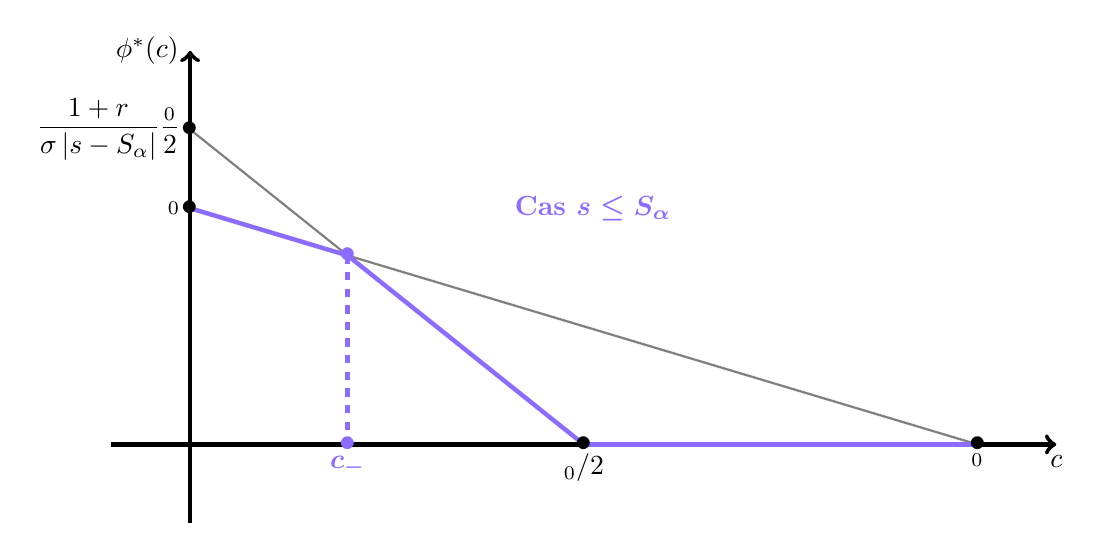
\begin{tikzpicture}

\draw [->, ultra thick] (-1, 0) -- (11, 0) node [below] {$c$};
\draw [->, ultra thick] (0, -1) -- (0, 5) node [left] {$\phi^*(c)$};

\draw [thick, gray] (0, 3) -- (10, 0);
\draw [thick, gray] (0, 4) -- (5, 0);

\draw [ultra thick, awesomePurple] (0, 3) -- (2, 2.4);
\draw [ultra thick, awesomePurple] (2, 2.4) -- (5, 0);
\draw [ultra thick, awesomePurple] (5, 0) -- (10, 0);

\node at (2, 2.4) {\color{awesomePurple}\large$\bullet$};
\draw [ultra thick, awesomePurple, dashed] (2, 2.4) -- (2, 0) node[below]{\color{awesomePurple}$\boldsymbol{c_-}$};

\node at (5, 0) {\large$\bullet$};
\node at (5, 0) [below] {$\W_0/2$};

\node at (10, 0) {\large$\bullet$};
\node at (10, 0) [below] {$\W_0$};

\node at (0, 3) {\large$\bullet$};
\node at (0, 3) [left] {$\W_0$};

\node at (2, 0) {\textbf{\color{awesomePurple}\large$\bullet$}};

\node at (0, 4) {\large$\bullet$};
\node at (0, 4) [left] {$\displaystyle{\frac{1+r}{\sigma\left|s - S_\alpha\right|}\frac{\W_0}{2}}$};

\node at (4, 3) [right] {\textbf{\color{awesomePurple}Cas $\boldsymbol{s\leq S_\alpha}$}};

\end{tikzpicture}

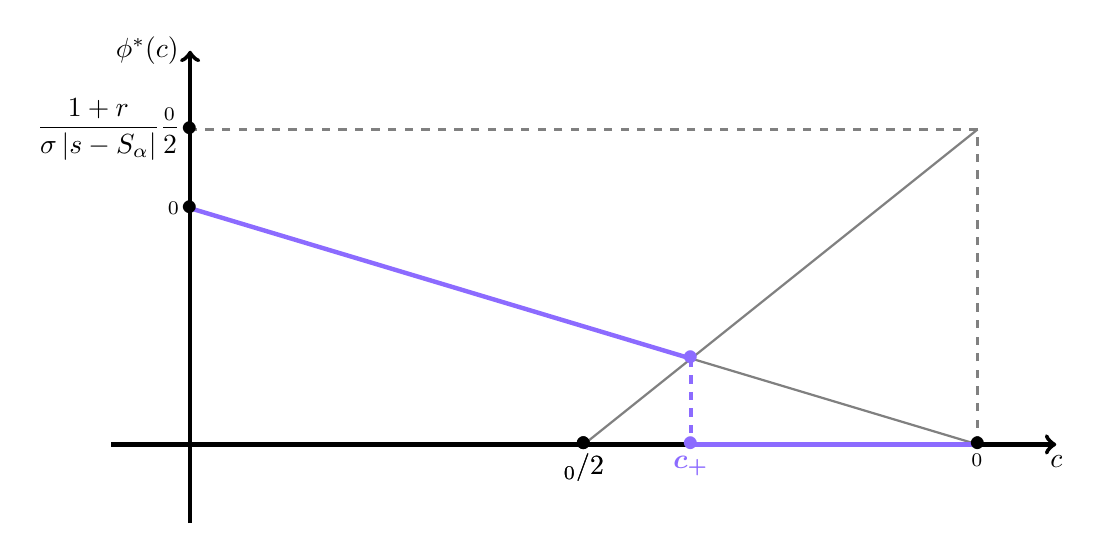
\begin{tikzpicture}

\draw [->, ultra thick] (-1, 0) -- (11, 0) node [below] {$c$};
\draw [->, ultra thick] (0, -1) -- (0, 5) node [left] {$\phi^*(c)$};

\draw [thick, gray] (0, 3) -- (10, 0);
\draw [thick, gray] (10, 4) -- (5, 0);
\draw [thick, gray, dashed] (10, 4) -- (0, 4);
\draw [thick, gray, dashed] (10, 0) -- (10, 4);

\draw [ultra thick, awesomePurple] (0, 3) -- (6.36, 1.09);
\draw [ultra thick, awesomePurple] (6.36, 0) -- (10, 0);

\node at (6.36, 1.09) {\color{awesomePurple}\large$\bullet$};
\draw [ultra thick, awesomePurple, dashed] (6.36, 1.09) -- (6.36, 0) node[below]{\color{awesomePurple}$\boldsymbol{c_+}$};

\node at (5, 0) {\large$\bullet$};
\node at (5, 0) [below] {$\W_0/2$};

\node at (10, 0) {\large$\bullet$};
\node at (10, 0) [below] {$\W_0$};

\node at (0, 3) {\large$\bullet$};
\node at (0, 3) [left] {$\W_0$};

\node at (0, 4) {\large$\bullet$};
\node at (0, 4) [left] {$\displaystyle{\frac{1+r}{\sigma\left|s - S_\alpha\right|}\frac{\W_0}{2}}$};

\node at (5, 0) {\large$\bullet$};
\node at (5, 0) [below] {$\W_0/2$};

\node at (6.36, 0) {\textbf{\color{awesomePurple}\large$\bullet$}};

\end{tikzpicture}
\caption{L'allocation optimale en actif risqué comme fonction de la consommation $c$}
\label{fig:allocation-optim}
\end{figure}

\paragraph{Deux cas distincts d'investissements.} Deux cas de figure se présentent, déterminés par la valeur de $s$ par rapport à $S_\alpha$. Avant de les développer, rappelons que l'on a en toute circonstance $0\leq \psi\leq \W_0 - c$.
\begin{itemize}
\item\textbf{Cas $\boldsymbol{s\leq S_\alpha}$: l'actif ne performe pas assez pour l'investisseur.}

Pour faire apparaitre une borne supérieure positive (cela permettra de diviser ensuite), on inverse le signe de l'inégalité après avoir multiplié les deux membres par $-1$. L'inégalité \eqref{eq:risk-ineq} devient 
$$
\frac{1+r}{\sigma\left(S_\alpha - s\right)}\left( \frac{\W_0}{2} - c \right) \geq \psi
$$
ce qui donne la condition générale pour la satisfaction des attentes en risques
\begin{equation}\label{eq:cond1}
0\leq\psi\leq \min\left( \W_0 - c, \frac{1+r}{\sigma\left(S_\alpha - s\right)}\left( \frac{\W_0}{2} - c \right) \right)
\end{equation}
en incluant la condition de conservation $\psi\leq\W_0-c$.

\item\textbf{Cas $s\geq S_\alpha$: l'actif a une performance intéressante pour l'investisseur} 

La borne supérieure est déjà positive, donc une rapide manipulation des termes transforme l'inégalité \eqref{eq:risk-ineq} en
$$
\frac{1+r}{\sigma\left(s - S_\alpha\right)}\left( c  - \frac{\W_0}{2}\right) \leq \psi
$$
et l'on conclut donc que les contraintes de conservation et d'aversion au risque seront satisfaites tant que
\begin{equation}\label{eq:cond2}
\frac{1+r}{\sigma\left(s - S_\alpha\right)}\left( c  - \frac{\W_0}{2}\right) \leq \psi\leq \W_0 - c.
\end{equation}
\end{itemize}

Comme évoqué à la section précédente, la nature linéaire en $\psi$ de la fonction objectif implique que l'on sature les contraintes aux bornes supérieures dans les inégalités \eqref{eq:cond1} et \eqref{eq:cond2}. On peut alors tracer l'allocation optimale $\phi^*(c)$ en fonction de la consommation $c$ (figure \ref{fig:allocation-optim}) à partir de l'équation

\begin{equation}
\phi^*(c) = \left\{ 
\begin{matrix}
\displaystyle{ \min\left[ \W_0 - c, \frac{1+r}{\sigma\left(S_\alpha - s\right)}\left( \frac{\W_0}{2} - c \right) \right]^+} & \textnormal{(si }s< S_\alpha\textnormal{)}\\
~&~\\
\displaystyle{\left(\W_0 - c\right)} \textnormal{ pour } c<c_+ \textnormal{ et } 0  \textnormal{ sinon}& \textnormal{(si }s< S_\alpha\textnormal{)} \\
\end{matrix}
\right.
\end{equation}
où l'exposant $+$ signifie $x^+ = \max(0, x)$.

\subsubsection{Quelques remarques sur la stratégie optimale d'investissement}

\begin{itemize}
\item Pour des ratios de Sharpe plus petit que le niveau exigé par l'aversion au risque du porteur, il est inutile d'investir dans l'actif risqué si l'on consomme $c = \W_0/2$ dès le début.\\

\textbf{\color{awesomePurple}Ce qui confirme que l'on peut difficilement battre le marché avec cette stratégie.}\\

En revanche, si l'on est patient et que l'on consomme moins, on peut s'attendre à un coupon plus important en période 1 et au global, pourvu que $m>r$, on peut espérer faire un gain total actualisé plus important que $\W_0$ avec une probabilité $\pi$ égale à
\begin{equation}
\pi = \N\left( -s \right) > \frac{1}{2}
\end{equation}

\textbf{\color{awesomePurple}Seule la patience permet de créer du levier grâce à une prise de risque maîtrisée.}\\

\item Pour des ratios de Sharpe plus petit que le niveau exigé par l'aversion au risque du porteur, il est possible de consommer jusqu'à 
\begin{equation}
c_+ = \frac{1 + r + 2\sigma\left( s - S_\alpha \right)}{1 + r + \sigma\left( s - S_\alpha \right)}\frac{W_0}{2}> \frac{W_0}{2}
\end{equation}
dès le début de l'investissement\footnote{La valeur $c_+$ est facilement obtenue en égalisant les bornes de l'inégalité \eqref{eq:cond2}.}.\\

C'est bien visible sur le schéma du bas sur la figure \ref{fig:allocation-optim}. Et cela s'explique par la sur-performance de l'actif qui augmente significativement les chances de rendement $\mu$ plus grands que $r$. La probabilité de $\mu>r$ est d'ailleurs égale à $\pi$ comme au cas précedent. A titre d'exemple, pour un $s$ qui serait plus grand que $1.96$ (quantile à 5\% de la distribution normale centrée réduite), cette probabilité est de 95\%.\\

Si l'on s'intéresse aux ordres de grandeur, on se rend vite compte que cette situation est en fait plutôt rarissime. Pour un niveau $\alpha = 5\%$, il faudrait que l'actif risqué ait un ratio de sharpe de plus de 1.96...\\

\end{itemize}

\section{Cas multipériodes.}\label{sec:multiperiodes}

Mettons-nous à présent dans la peau d'un petit porteur qui a (toujours) à sa disposition un capital $\W_0$ à l'instant $0$. Il cherche à savoir comment il pourrait allouer son capital entre un actif risqué (de même nature que celui présenté précédemment) et un actif sans risque (lui aussi de même nature) \textbf{\color{awesomePurple} à chaque période $\boldsymbol{k = 0\dots (K - 1)}$}.\\

Trouver une stratégie optimale d'investissement au cas multipériodes n'est pas si simple et requiert une généralisation du raisonnement fait précedemment qui sera présenté à la prochaine section. En substance, il s'agira de considérer qu'à chaque période où il alloue son capital, il raisonnera comme s'il était sur une période en deux temps.

\subsection{Le modèle}

Le modèle des flux financiers n'est qu'une réécriture séquentielle de ce qui a été décrit à la section \ref{sec:deux-periodes-model}. Il n'y a donc pas de grande surprise, il s'agit simplement de mettre des indices $k$ sur l'ensemble des variables pour caractériser les grandeurs à l'instant $k$ (voir figure \ref{fig:flux-de-richesse-k-k+1}).\\

\subsection{Les variables}

D'après la figure \ref{fig:flux-de-richesse-k-k+1}, le petit porteur place en l'instant $k$ 
\begin{itemize}
\item une valeur $\psi_k$ dans l'actif risqué;
\item une valeur $\psi^0_k$ dans l'actif sans risque.
\end{itemize}
Il consomme également $c_k$, de sorte que sa richesse en $k$, $\W_k$, peut s'exprimer comme la somme de $\psi_k$, $\psi^0_k$ et de $c_k$
\begin{equation}\label{eq:conservation-k}
\W_k = \psi_k + \psi^0_k + c_k.
\end{equation}
En l'instant $(k + 1)$, il reçoit 
\begin{itemize}
\item une valeur $(1 + \mu_k)\psi_k$ de son placement risqué;
\item une valeur $(1 + r)\psi_k^0$ de son placement sans risque.
\end{itemize}
Il fait le choix de réinvestir suivant la même stratégie jusqu'en $K - 1$ (inclus) et à l'instant $K$, il arrête son investissement.\\

On considère les $\mu_k$ comme des variables gaussiennes indépendantes\footnote{Cette hypothèse est très forte et nécessiterait en premier lieu d'être modifiée au profit d'un modèle à volatilité stochastique.} de moyenne $m$ et de variance $\sigma^2$. On écrira donc 
$$
\mu_k = m + \sigma\epsilon_k.
$$

\begin{figure}[h!]
\centering
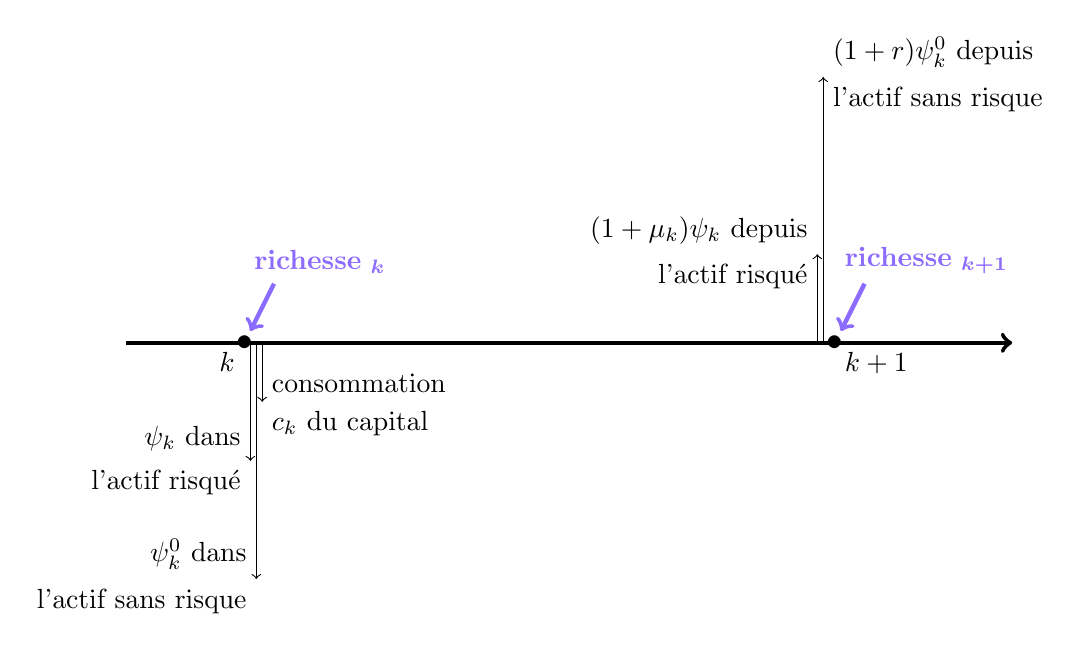
\begin{tikzpicture}[scale = .75]
\draw[->, ultra thick] (-2, 0) -- (13, 0);

\node at (0, 0) {\large $\bullet$};
\node at (0, 0) [below left] {$k$};
\node at (0, 1) [above right] {\color{awesomePurple}\textbf {richesse} $\boldsymbol {\W_{k}}$};
\draw [->, ultra thick, awesomePurple] (.5, 1) -- (0.1, .2);

\node at (10, 0) {\large$\bullet$};
\node at (10, 0) [below right] {$k + 1$};
\node at (10, 1) [above right] {\color{awesomePurple}\textbf {richesse} $\boldsymbol {\W_{k + 1}}$};
\draw [->, ultra thick, awesomePurple] (10.5, 1) -- (10.1, .2);

\draw[->] (0.1, 0) -- (0.1, - 2);
\node at (0.1, -2) [above left] {$\psi_k$ dans};
\node at (0.1, -2) [below left] {l'actif risqué};

\draw[->] (.2, 0) -- (.2, - 4);
\node at (.2, -4) [above left] {$\psi^0_k$ dans};
\node at (.2, -4) [below left] {l'actif sans risque};

\draw[->] (.3, 0) -- (.3, - 1);
\node at (.3, -1) [above right] {consommation};
\node at (.3, -1) [below right] {$c_k$ du capital};


\draw[->] (9.7, 0) -- (9.7, 1.5);
\node at (9.7, 1.5) [above left] {$(1 + \mu_k)\psi_k$ depuis};
\node at (9.7, 1.5) [below left] {l'actif risqué};

\draw[->] (9.8, 0) -- (9.8, 4.5);
\node at (9.8, 4.5) [above right] {$(1 + r)\psi_k^0$ depuis};
\node at (9.8, 4.5) [below right] {l'actif sans risque};

\end{tikzpicture}
\caption{Les flux de richesse entre deux instant de gestion $k$ et $k + 1$.}
\label{fig:flux-de-richesse-k-k+1}
\end{figure}


En substance, après quelques calculs sur les flux, on obtient que 
\begin{itemize}
\item la variation de richesse $\tilde\W$ entre $k$ et $k+1$ (actualisée en $0$) s'écrit
$$
\tilde\W_{k + 1} - \tilde\W_k = \frac{\mu_k - r}{(1 + r)^{k + 1}}\psi_k - \frac{c_k}{(1 + r)^k};
$$
\item la richesse finale actualisée $\tilde \W_K$ est obtenue après un sommage télescopique
$$
\tilde \W_K = W_0 + \sum_{k = 0}^{K - 1}\frac{\mu_k - r}{(1 + r)^{k + 1}}\psi_k - \sum_{k = 0}^{K - 1}\frac{c_k}{(1 + r)^k};
$$
\item le gain actualisé $\tilde \G_K$, qui n'est autre que $\tilde \W_K$ plus les flux de coupons $c_k$ actualisés en 0 eux aussi, s'obtient immédiatement comme
$$
\tilde \G_K = W_0 + \sum_{k = 0}^{K - 1}\frac{\mu_k - r}{(1 + r)^{k + 1}}\psi_k.
$$
\end{itemize}

Tout s'est formules reviennent bien entendu aux mêmes que celle obtenue en première section en prenant $K = 1$.

\subsection{Stratégie d'investissement du petit porteur avec mises répétées.}

Dans un cas multipériode, on pourrait considérer que le petit porteur ajuste sa stratégie au fur et à mesure, modifiant les quantités placées dans l'actif risqué ainsi que le coupon qu'il se verse. Avec cette approche il pourrait gérer son risque au mieux et en temps réel.\\

Néanmoins, dans une optique directionnelle où une cotation suit un trend de marché considéré stable, le petit porteur peut adopter une stratégie actualisée de placement en actif risqué $\phi(c)$ indépendante du temps. On cherchera donc des stratégies de la forme
$$
\psi_k = \left(1 + r\right)^k\phi\left( c \right)
$$
où $c_k = (1 + r)^k c$.

\subsubsection{Objectif d'investissement.}

Comme dans le cas monopériode, le porteur souhaite maximiser ses revenus totaux actualisés en zéro et donc la fonction objectif n'est autre que $\tilde\G_K - W_0$. Il est conduit à chercher une solution au problème
\begin{equation}
\max_{\psi_k, c_k}\sum_{k = 0}^{K - 1}\frac{\mu_k - r}{(1 + r)^{k + 1}}\psi_k.
\end{equation}
qui est une nouvelle fois linéaire en la stratégie d'investissement. Ce seront donc les contraintes d'aversion au risque du porteur qui permettront de déterminer la solution $\phi^*(c)$ et saturant ces dernières. Et une fois la forme de la solution calculée, il s'agira de lui trouver son maximum en fonction du coupon actualisé.

\subsubsection{Choix de la mesure de risque.} 

Comme dans le cas mono-période, le porteur part du principe qu'il pourrait placer son capital dans l'actif sans risque et récupérer un coupon 
\begin{equation}
(1 + r)^k\frac{\W_0}{K + 1}.
\end{equation}

S'il utilise cette stratégie de placement, sa richesse actualisée à zéro est amortie linéairement et en tout instant $k$ elle vaut
\begin{equation}
\left( 1 - \frac{k}{K + 1}\right)\W_0 =\frac{K - k + 1}{K + 1}\W_0.
\end{equation}

\textbf{\color{awesomePurple}De son point de vue, prendre des risques n'a de sens que s'il peut avoir une certaine maîtrise sur la probabilité de sous-performer par rapport à cette stratégie sans risque.}\\

Mathématiquement, on exprimera son aversion au risque comme
\begin{equation}\label{eq:risk-ineq-raw-multi}
\mathds P\left[ \left(\tilde\W_1\geq\frac{K}{K + 1}\W_0\right)\wedge \dots\wedge \left(\tilde\W_k\geq\frac{K - k + 1}{K + 1}\W_0\right)\wedge \dots\wedge \left(\tilde\W_K\geq\frac{1}{K + 1}\W_0\right) \right] \geq 1 - A
\end{equation}
où $A$ est une borne supérieure à la probabilité qu'il fasse moins bien que le placement sans risque à une période au moins.\\

L'expression ci-dessus signifie que le porteur s'attend, en chaque période, à avoir une richesse actualisée supérieure à celle qu'il aurait eu avec le placement sans risque. Les bornes inférieures des inégalités sur les richesses actualisées expriment exactement que le niveau de richesse en $k$ est plus important que celui qu'il aurait acquis avec le placement sans risque.

\subsubsection{Généralisation de la stratégie optimale $\phi^*(c)$.}

Pour calculer $\phi^*(c)$, on peut utiliser plusieurs méthodes. Une première appoche consisterait à exprimer analytiquement l'inégalité \eqref{eq:risk-ineq-raw-multi} puis calculer sa valeurs pour des points de l'espace des phases $(c, \psi)$. Une seconde approche utiliserait une méthode de Monte-Carlo pour tracer un nuage de points dans ce même espace des phases.

\paragraph{Méthode de calcul choisie.} On optera pour la seconde méthode. La première demandant elle-même possiblement l'implémentation d'une méthode de Monte-Carlo pour le calcul d'une intégrale\footnote{Succinctement, le processus $(\tilde\W_k)$ est une chaîne de Markov et on a
\begin{equation*}
\begin{split}
\mathds P\left[ \left(\dots\wedge \left(\tilde\W_k\geq\frac{K - k + 1}{K + 1}\W_0\right)\wedge \dots\right) \right] &= \left[\prod_{k = 1}^{K - 1} \mathds P\left( \left. \tilde\W_{k+1}\geq\frac{K - k}{K + 1}\W_0 \right| \tilde\W_k\geq\frac{K - k + 1}{K + 1}\W_0 \right)\right]P\left( \tilde\W_{1}\geq\frac{K}{K + 1}\W_0\right)\\
&= \left[\prod_{k = 1}^{K - 1} \int_{\frac{K - k + 1}{K + 1}\W_0}^{+\infty}\mathds P\left( \left. \tilde\W_{k+1}\geq\frac{K - k}{K + 1}\W_0 \right| \tilde\W_k=\tilde w_k \right) p\left(\tilde w_k\right) \diff\tilde w_k\right]P\left( \tilde\W_{1}\geq\frac{K}{K + 1}\W_0\right)\\
\end{split}
\end{equation*}
\noindent l'intégrande dans le produit a une expression analytique qui fait intervenir la fonction de répartition de la loi gaussienne $\N$, mais l'intégrale doit être évaluée numériquement. Une méthode de Monte-Carlo offre la voie la plus directe et la moins complexe pour y parvenir...
}.

\paragraph{La richesse du porteur est une marche aléatoire contrainte.} La nature stochastique de la gestion de l'investissement vient du caractère aléatoire de la variation du prix de l'actif risqué. Naturellement, un portefeuille qui contiendrait un tel actif serait nécessairement aléatoire lui aussi.\\

Pour rappel, les rendements de l'actif risqué aux instants $k$ sont donnés par
$
\mu_k = m + \sigma \epsilon_k
$
où les $\epsilon_k$ sont des variables gaussiennes centrées réduites indépendantes. Le processus des richesses actualisées en zéro du petit porteur est définit par la relation de récurrence
\begin{equation*}
\begin{split}
\tilde \W_0 &=  \W_0\\
\tilde\W_{k + 1} &= \tilde\W_k + \frac{\mu_k - r}{(1 + r)}\phi(c) - c.
\end{split}
\end{equation*}
Dans le cadre fixé par ce modèle, la richesse du porteur et une marche aléatoire gaussienne de drift 
$$
\frac{m - r}{(1 + r)}\phi(c) - c
$$
et d'écart type
$$
\frac{\sigma}{(1 + r)}\phi(c).
$$\\

\textbf{\color{awesomePurple}Il est à noter que le drift du processus n'a pas à être positif et que le risque pris par le porteur dépend directement de la stratégie (dpéendance linaire avec l'écart-type).}\\

Concernant le dift, s'il est positif, tant mieux. S'il ne l'est pas, n'oublions pas que le porteur souhaite se verser ``intelligement'' un coupon sur une mise initiale. Sa richesse est donc vouée à décliner.\\

Dans la section précédente, on évoquait une contrainte de conservation telle que 
$$
0\leq\psi_0 \leq \W_0 + c.
$$
Dans le cas multipériode présent, cette contrainte ce généralise en
$$
0\leq\psi_k\leq\W_k + c_k,
$$
ce qui, en incluant les formes cherchées pour $\psi_k = (1 + r)^k\phi$ et $c_k = (1 + r)^k$ s'écrit
\begin{equation}
0\leq\phi\leq\tilde\W_k + c.
\end{equation}
Aussi, si à un instant $k$, la fortune $\tilde\W_k$ atteint 0, alors pour tout instant ultérieur, cette fortune reste nulle. C'est la ruine du joueur.\\

On adapte alors la dynamique de la marche aléatoire en prenant en compte ces deux contraintes (contrainte de conservation et contrainte de ruine) avec la dynamique suivante.
\begin{equation*}
\begin{split}
\tilde \W_0 &=  \W_0\\
\tilde\W_{k + 1} &= \max\left[0, \tilde\W_k + \frac{\mu_k - r}{(1 + r)}\min\left(\phi(c), \tilde\W_k - c\right) - c\right].
\end{split}
\end{equation*}

\paragraph{Méthode de Monte-Carlo.} Sans rentrer dans trop de détails, la méthode de Monte-Carlo consiste à simuler une multitude de chemins dont le nombre $S$ est bien souvent de l'ordre du million voire du milliard quand cela est possible. Il arrive que pour des systèmes très complexes, le nombre de simulations tombe à quelques milliers ou centaines.\\

Avec toutes ces trajectoires, on peut calculer la mesure du risque du petit porteur et évaluer la valeur $\phi(c)$  qui assurera un retour sur investissement maximum en l'actif risqué.







\end{document}